\documentclass{article}
\usepackage{tikz}
\usepackage{graphicx}
\usepackage{fontspec}
\usetikzlibrary{positioning, shapes.geometric, arrows, calc,fit,backgrounds}


% Ορισμός ενός στυλ για έντονη γραμματοσειρά
\tikzset{myTextStyle/.style={font=\bfseries\fontspec{Arial}}}

\begin{document}
	
	\begin{figure}[htbp]
		\centering
		\resizebox{\textwidth}{!}{
			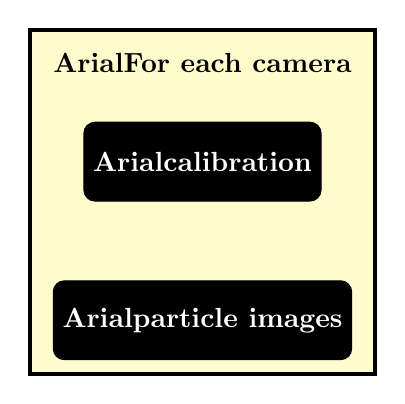
\begin{tikzpicture}
				% Nodes
				\node (calibration) [rectangle, minimum width=3cm, minimum height=1cm, text centered, draw=black, rounded corners, fill=black, text=white, myTextStyle] {calibration};
				\node (particleimages) [rectangle, minimum width=3cm, minimum height=1cm, text centered, draw=black, rounded corners, fill=black, text=white, below=of calibration, myTextStyle] {particle images};
				
				% Label inside the fitbox at the top
				\node (label) [above=0.5cm of calibration, text=black, text depth=0, myTextStyle] {\textbf{For each camera}};
				
				% Fit box with a stroke (border)
				\begin{scope}[on background layer]
					\node [draw=black, line width=1.5pt, inner sep=5pt, fill=yellow!20, fit=(label) (calibration) (particleimages)] (fitbox) {};
				\end{scope}
			\end{tikzpicture}
			
			
			
			\begin{tikzpicture}[node distance=1cm]
				
				
				
				\node (volume) [
				rectangle,
				minimum width=3cm,
				minimum height=1cm,
				text centered,
				draw=black,
				rounded corners,
				fill=black,
				text=white,
				below=3.5cm of calibration,
				right=3.5cm of $(calibration)!0.5!(particleimages)$,
				align=center, myTextStyle 
				] {volume self \\ Calibration};
				
				
				
				\node (otf) [
				rectangle, 
				minimum width=3cm, 
				minimum height=1cm, 
				text centered, 
				draw=black, 
				rounded corners, 
				fill=black, 
				text=white, 
				right=of volume,
				align=center, myTextStyle
				] {optical transfer \\ function};
				
				
				\node (tomographic) [
				rectangle, 
				minimum width=3cm, 
				minimum height=1cm, 
				text centered, 
				draw=black, 
				rounded corners, 
				fill=black, 
				text=white, 
				above right=0.15cm and 1.5cm of otf,
				align=center, myTextStyle
				] {tomographic \\ reconstruction};
				
				\node (triangulation) [
				rectangle, 
				minimum width=3cm, 
				minimum height=1cm, 
				text centered, 
				draw=black, 
				rounded corners, 
				fill=black, 
				text=white, 
				below right=0.15cm and 1.5cm of otf,
				align=center, myTextStyle 
				] {triangulation/ \\ IPR};
				
				
				\node (cross) [
				rectangle, 
				minimum width=3cm, 
				minimum height=1cm, 
				text centered, 
				draw=black, 
				rounded corners, 
				fill=black, 
				text=white, 
				right=of tomographic,
				align=center, myTextStyle 
				] {3D cross- \\ correlation};
				
				\node (tracking) [
				rectangle, 
				minimum width=3cm, 
				minimum height=1cm, 
				text centered, 
				draw=black, 
				rounded corners, 
				fill=black, 
				text=white, 
				right=of triangulation,
				align=center, myTextStyle 
				] {3D Tracking};
				
				\node (velocity) [
				rectangle, 
				minimum width=3cm, 
				minimum height=1cm, 
				text centered, 
				draw=black, 
				rounded corners, 
				fill=black, 
				text=white, 
				below=3.5cm of cross, 
				right=3.5cm of $(cross)!0.5!(tracking)$, myTextStyle
				] {3D3C velocity field};
				
				% Arrows
				\draw [thick,gray,->,>=stealth,line width=3.5pt] (calibration) -- (volume);
				\draw [thick,gray,->,>=stealth,line width=3.5pt] (particleimages) -- (volume);
				\draw [thick,gray,->,>=stealth,line width=3.5pt] (volume) -- (otf);
				\draw [thick,gray,->,>=stealth,line width=3.5pt] (otf) -- (tomographic);
				\draw [thick,gray,->,>=stealth,line width=3.5pt] (otf) -- (triangulation);
				\draw [thick,gray,->,>=stealth,line width=3.5pt] (tomographic) -- (cross);
				\draw [thick,gray,->,>=stealth,line width=3.5pt] (triangulation) -- (tracking);
				\draw [thick,gray,->,>=stealth,line width=3.5pt] (cross) -- (velocity);
				\draw [thick,gray,->,>=stealth,line width=3.5pt] (tracking) -- (velocity);
				
			\end{tikzpicture}
		}
		\caption{A schematic of different steps in a 3D PIV/RTV measurement}
		\label{fig:pipeline}
	\end{figure}
	
\end{document}
